\section{Tecnologias}

O desenvolvimento do sistema \textbf{Tropical Mix} foi estruturado a partir de um conjunto de tecnologias modernas e amplamente utilizadas no mercado de desenvolvimento web. A escolha das ferramentas considerou critérios como desempenho, escalabilidade, segurança e facilidade de manutenção. A seguir, são descritas as principais tecnologias aplicadas em cada camada da aplicação.

\subsection{Front-end}

A camada de \textit{front-end} do sistema foi desenvolvida utilizando a biblioteca \textbf{React.js}, que possibilita a criação de interfaces de usuário modernas, dinâmicas e responsivas. Essa tecnologia, baseada em componentes reutilizáveis, permite a construção de telas interativas e modulares, facilitando a manutenção e a evolução da aplicação.  

A escolha pelo React deve-se à sua eficiência no gerenciamento do estado da aplicação, à sua capacidade de atualização em tempo real e à ampla comunidade de desenvolvedores, o que assegura suporte contínuo e uma vasta gama de bibliotecas complementares.  

Para a estruturação e estilização das páginas, foram utilizadas as tecnologias \textbf{HTML5} e \textbf{CSS3}, permitindo a criação de layouts responsivos que se adaptam a diferentes dispositivos, como computadores, tablets e smartphones. A comunicação entre o \textit{front-end} e o \textit{back-end} é realizada por meio de requisições HTTP utilizando a biblioteca \textbf{Axios}, que possibilita a troca de dados de forma assíncrona e eficiente.  

Além das funcionalidades de navegação e controle de estoque e vendas, o \textit{front-end} também inclui o módulo de geração de relatórios com informações temporais em relação aos indicadores de desempenho do cliente. Esse painel consome dados disponibilizados pela API do \textit{back-end} e apresenta informações estratégicas, como volume de vendas, produtos com menor estoque e desempenho por período, em gráficos e tabelas dinâmicas.  

Dessa forma, o \textit{front-end} não apenas oferece uma interface intuitiva e agradável ao usuário, mas também serve como ferramenta de apoio à gestão, centralizando visualmente as informações mais relevantes para a tomada de decisão.

\subsection{Back-end}

O \textit{back-end} foi implementado utilizando a linguagem \textbf{Python}, em conjunto com o microframework \textbf{Flask}, responsável por gerenciar as rotas, processar as regras de negócio e realizar a comunicação com o banco de dados. O Flask foi escolhido por sua leveza, flexibilidade e fácil integração com outras tecnologias, além de oferecer suporte nativo à construção de APIs RESTful.  

Entre as principais funcionalidades desenvolvidas nessa camada, destacam-se:
\begin{itemize}
    \item Gerenciamento de usuários e autenticação, com controle de perfis de acesso;
    \item Registro e controle de vendas e movimentações de estoque;
    \item Processamento de dados para geração de relatórios e indicadores exibidos nas páginas do \textit{front-end};
    \item Integração com o banco de dados \textbf{MySQL} para armazenamento e consulta das informações.
\end{itemize}

O uso do Flask proporciona um desenvolvimento ágil, modular e seguro, permitindo que novas funcionalidades sejam incorporadas de forma independente, sem comprometer a arquitetura do sistema. A comunicação com o \textit{front-end} ocorre por meio de uma \textbf{API REST}, garantindo a troca estruturada e eficiente de dados no formato \textbf{JSON}.


\subsection{Banco de Dados}

O banco de dados escolhido para o sistema é o \textbf{MySQL}, um dos gerenciadores de banco de dados relacionais mais consolidados no mercado. Sua escolha foi motivada pela confiabilidade, escalabilidade e ampla compatibilidade com aplicações baseadas em Python.  

O modelo de dados foi projetado de forma a garantir integridade referencial e desempenho nas operações de leitura e escrita. Cada transação, seja de venda, compra ou atualização de estoque, é registrada no banco de dados, permitindo o acompanhamento detalhado das atividades da loja.  

Além disso, a estrutura relacional do MySQL possibilita consultas otimizadas para a geração de relatórios, facilitando a análise de dados e o processo de tomada de decisão por parte da gestão da \textbf{Tropical Mix}.



\subsection{Infraestrutura}

A infraestrutura usada para o sistema Tropical Mix visa garantir estabilidade e segurança ao ambiente de execução da aplicação. Durante o desenvolvimento, a aplicação será executada em ambiente local pelos integrantes da equipe, utilizando servidores Flask para o back-end e o serviço de hospedagem local do React para o front-end.

Para a fase de implantação, utilizamos o serviço de computação em nuvem, \textbf{Amazon Web Services (AWS)} que oferece planos gratuitos e compatíveis com aplicações em Flask e React. O banco de dados MySQL vai ser hospedado no serviço \textbf{Amazon RDS}, garantindo persistência remota e acessibilidade para todos os desenvolvedores.

A arquitetura proposta segue o modelo cliente-servidor, em que o front-end (cliente) se comunica com o back-end (servidor Flask) via API REST, como mostra a Figura~\ref{fig:cliente-servidor}. O ambiente de nuvem permitirá a configuração de endpoints públicos e o gerenciamento de logs, autenticação e escalabilidade sob demanda.

\begin{figure}[H]
  \centering
  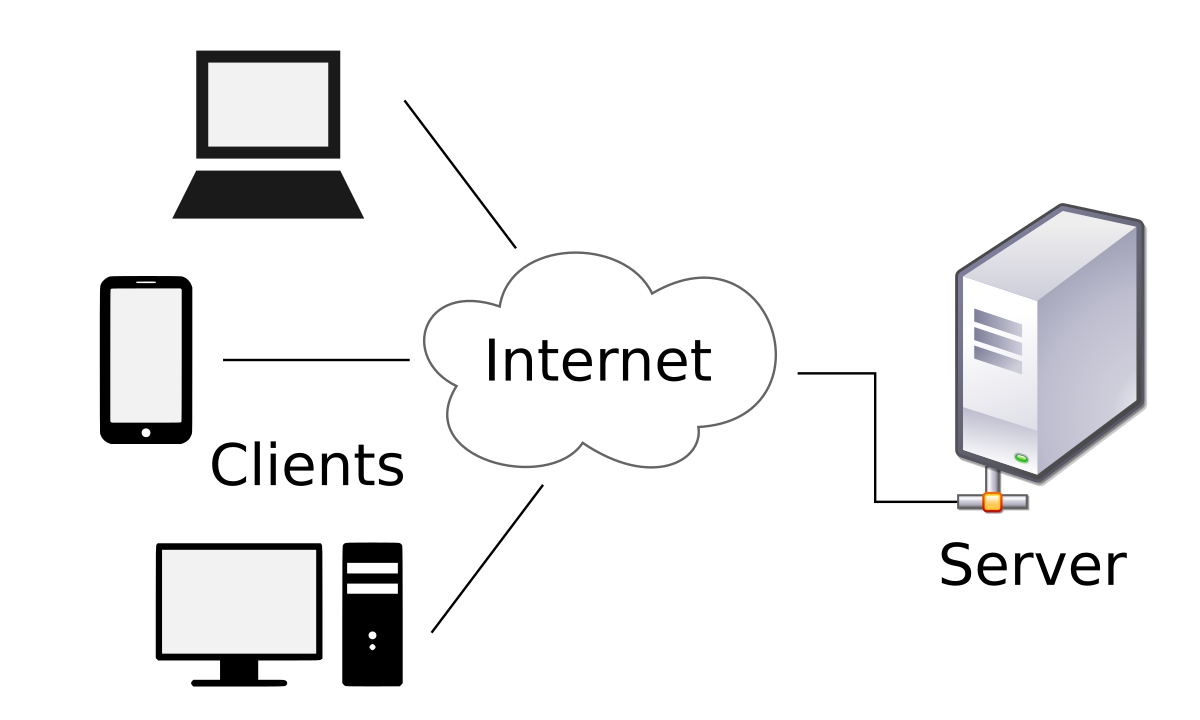
\includegraphics[width=0.9\textwidth]{documentacao/LaTex/Capítulos/img/Desenvolvimento do Projeto/Arquitetura/cliente-servidor.png}
  \caption{Arquitetura Cliente-Servidor.}
  \fonte{SAMPAIO, Guilherme. \textit{Introdução à Arquitetura Cliente-Servidor}. Medium, 2021. Disponível em: https://medium.com/@kaisergui258/introdução-a-arquitetura-cliente-servidor-dfae4c0218bd. Acesso em: 27 de outubro de 2025 }
  \label{fig:cliente-servidor}
\end{figure}




\subsection{Ferramentas de Apoio}

Durante o desenvolvimento do sistema, foram utilizadas diversas ferramentas de apoio para gerenciar as etapas do projeto, promover a colaboração entre os integrantes e garantir a qualidade do código. A Tabela~\ref{tab:ferramentas-apoio} apresenta um resumo das principais ferramentas adotadas.

\begin{table}[H]
\centering
\caption{Ferramentas de apoio utilizadas}
\label{tab:ferramentas-apoio}
\begin{tabular}{|p{3cm}|p{11cm}|}
\hline
\textbf{Ferramenta} & \textbf{Descrição} \\ \hline

\textbf{GitHub} & Plataforma de hospedagem de código-fonte utilizada para controle de versão, colaboração entre desenvolvedores e gerenciamento das alterações do sistema. O GitHub também foi integrado ao Kanban para acompanhamento das tarefas em tempo real. \\ \hline

\textbf{Notion} & Ferramenta colaborativa voltada para documentação e planejamento. Foi utilizada para registrar decisões de projeto, anotações de reuniões e controle de cronogramas de atividades. \\ \hline

\textbf{Overleaf} & Plataforma online para edição de documentos em Latex, utilizada para a elaboração e padronização do relatório técnico e do Projeto de Conclusão de Curso(PPC). Permitiu edição simultânea e controle de versões do texto. \\ \hline

\textbf{Google Meet} & Ferramenta de videoconferência usada para reuniões de acompanhamento e alinhamento das etapas do projeto entre os integrantes da equipe e o orientador. \\ \hline


\end{tabular}
\fonte{Elaborado pelos autores.}
\end{table}